\documentclass[t,xcolor=pdftex,dvipsnames,table]{beamer}
\usepackage[]{graphicx}\usepackage[]{color}
%% maxwidth is the original width if it is less than linewidth
%% otherwise use linewidth (to make sure the graphics do not exceed the margin)
\makeatletter
\def\maxwidth{ %
  \ifdim\Gin@nat@width>\linewidth
    \linewidth
  \else
    \Gin@nat@width
  \fi
}
\makeatother

\definecolor{fgcolor}{rgb}{0.345, 0.345, 0.345}
\newcommand{\hlnum}[1]{\textcolor[rgb]{0.686,0.059,0.569}{#1}}%
\newcommand{\hlstr}[1]{\textcolor[rgb]{0.192,0.494,0.8}{#1}}%
\newcommand{\hlcom}[1]{\textcolor[rgb]{0.678,0.584,0.686}{\textit{#1}}}%
\newcommand{\hlopt}[1]{\textcolor[rgb]{0,0,0}{#1}}%
\newcommand{\hlstd}[1]{\textcolor[rgb]{0.345,0.345,0.345}{#1}}%
\newcommand{\hlkwa}[1]{\textcolor[rgb]{0.161,0.373,0.58}{\textbf{#1}}}%
\newcommand{\hlkwb}[1]{\textcolor[rgb]{0.69,0.353,0.396}{#1}}%
\newcommand{\hlkwc}[1]{\textcolor[rgb]{0.333,0.667,0.333}{#1}}%
\newcommand{\hlkwd}[1]{\textcolor[rgb]{0.737,0.353,0.396}{\textbf{#1}}}%
\let\hlipl\hlkwb

\usepackage{framed}
\makeatletter
\newenvironment{kframe}{%
 \def\at@end@of@kframe{}%
 \ifinner\ifhmode%
  \def\at@end@of@kframe{\end{minipage}}%
  \begin{minipage}{\columnwidth}%
 \fi\fi%
 \def\FrameCommand##1{\hskip\@totalleftmargin \hskip-\fboxsep
 \colorbox{shadecolor}{##1}\hskip-\fboxsep
     % There is no \\@totalrightmargin, so:
     \hskip-\linewidth \hskip-\@totalleftmargin \hskip\columnwidth}%
 \MakeFramed {\advance\hsize-\width
   \@totalleftmargin\z@ \linewidth\hsize
   \@setminipage}}%
 {\par\unskip\endMakeFramed%
 \at@end@of@kframe}
\makeatother

\definecolor{shadecolor}{rgb}{.97, .97, .97}
\definecolor{messagecolor}{rgb}{0, 0, 0}
\definecolor{warningcolor}{rgb}{1, 0, 1}
\definecolor{errorcolor}{rgb}{1, 0, 0}
\newenvironment{knitrout}{}{} % an empty environment to be redefined in TeX

\usepackage{alltt}
\newcommand{\SweaveOpts}[1]{}  % do not interfere with LaTeX
\newcommand{\SweaveInput}[1]{} % because they are not real TeX commands
\newcommand{\Sexpr}[1]{}       % will only be parsed by R


%\documentclass[handout,t,xcolor=pdftex,dvipsnames,table]{beamer}  % For handout
\mode<presentation>{
\useoutertheme[subsection=false]{miniframes}
%\beamertemplatenavigationsymbolsempty
\usecolortheme{custom}
\usefonttheme[onlymath]{serif}
\setbeamercovered{invisible}
%\setbeamertemplate{navigation symbols}{}
%\setbeamertemplate{mini frames}{}  % Old one
% Comment out this line to give the header
% \setbeamertemplate{headline}[default]
\setbeamertemplate{caption}[numbered]
%\setbeamertemplate{itemize items}[circle] 
\setbeamertemplate{frametitle continuation}{\frametitle{\color{white}Title}}  % So no tile on subsequent frames, from [allowframebreaks]

%%% CUSTOMISING NAVIATION %%%%
%This customises the navigation to be thin width and just have section headings (not subsections). 
\setbeamertemplate{headline}{%
\leavevmode%
  \hbox{%
    \begin{beamercolorbox}[wd=\paperwidth,ht=2.5ex,dp=1.125ex]{palette tertiary}%   % Tertiary colour is blue
    \insertsectionnavigationhorizontal{\paperwidth}{}{\hskip0pt plus1filll}
    \end{beamercolorbox}%
}}}

\RequirePackage{marvosym}

%%% INCLUDING SOLUTIONS %%%%
%% You can incorporate both questions and solutions in the 
%% same document.  Solutions can be included between the 
%% commands \begin{soln} and \end{soln}
%% To generate a pdf with only the questions uncomment:
%\excludecomment{soln}
\usepackage{comment}
\specialcomment{soln}{\begingroup \vspace{1mm} \sl}{ \leavevmode \endgroup}

%%%% DETAILS FOR PART 1 TITLE PAGE (OLD) %%%%
%\title{\large Part2 - Probability \& Distribution Theory} 
%\subtitle{} 
%\author{\copyright Dr Di Warren 2016} 
%\date{MATH1005 - Statistics}
% \colorlet{Faculty}{Arts}
%\colorlet{Faculty}{MasterBrandRed} % This is only needed if the notes are used for different faculties.
%\colorlet{FacultyText}{White}
% Defines the color of the text used on the title page and ``blocks''
% White for Business; TitlePageBlack for Arts, Pharmacy and Science
%\definecolor{CoolBlack}{rgb}{0.0, 0.18, 0.39}

%%%% DETAILS FOR FULL COURSE TITLE PAGE %%%%
\title{\Huge STATISTICS} 
\subtitle{} 
\author{\copyright University of Sydney 2017 (Di Warren)} 
\date{MATH1005}
% \colorlet{Faculty}{Arts}
\colorlet{Faculty}{MasterBrandRed} % This is only needed if the notes are used for different faculties.
\colorlet{FacultyText}{White}
% Defines the color of the text used on the title page and ``blocks''
% White for Business; TitlePageBlack for Arts, Pharmacy and Science
\definecolor{CoolBlack}{rgb}{0.0, 0.18, 0.39}

%%%% PACKAGES %%%%
\usepackage{multirow}
\usepackage{fancybox}
\usepackage[english]{babel}
\usepackage[utf8]{inputenc}
\usepackage{bm}
\usepackage{array}
\usepackage{booktabs}
\usepackage{tikz}
\usetikzlibrary{matrix,arrows,decorations.pathmorphing}
\usepackage{verbatim}
\usepackage{pgf,pgfsys,pgffor}
\usepackage{pgfplots}
\pgfplotsset{compat=1.3} %Recommended as of Pgfplots 1.3 - necessary?
\usetikzlibrary{decorations.pathreplacing,calc}
\usetikzlibrary{shapes, backgrounds}   % For Venn diagrams
\def \setA{ (0,0) circle (1cm) }
\def \setB{ (1.5,0) circle (1cm) }
\def \setC{ (0.6,1.5) circle (1cm) }
\def \setO{ (-2, -1.5) rectangle (3.5, 2.75) }
\tikzstyle{every picture}+=[remember picture]
\tikzstyle{na} = [baseline=-.5ex]
\usepackage{listings}  %Added by Di for adding R code

%\AtBeginSection[]
%{
%   \begin{frame}
 %      \frametitle{Outline}
 %      \tableofcontents[currentsection]
%   \end{frame}
%}  %This seems overkill for weekly lecture slides.

%\AtBeginSection[]
%{
%  \begin{frame}
% \frametitle{Contents}
%  \tiny{\tableofcontents[currentsection]}
%  \end{frame}
%}
%\useoutertheme{infolines} % Just lists current section in navigation at top, nice but limiting?

%%%% TITLE PAGE AND CONTENTS AT BEGINNING OF EACH TOPIC %%%%

\RequirePackage{ifthen} % package required
\newboolean{sectiontoc}
\setboolean{sectiontoc}{true} %default to true

\AtBeginSection[]
{
\begin{frame}[plain]
\vspace{60pt}
\begin{center}
\Huge{{\textcolor{MasterBrandBlue} \insertsection}}
\end{center}
\begin{tikzpicture}[scale=0.54]
%\hspace{-12pt}
%% Big Rectangle
\fill[MasterBrandRed] (0,14) -- (20,14) -- (20,15) -- (0,15);

%\draw (1,14.5) node [anchor = west] {\textcolor{MasterBrandBlue}{\Huge{\insertsection}}}; Overlays box with title, but long titles drop off the page
\end{tikzpicture} 
\end{frame}

%%%%%WORKING VERSION OF TOC%%%%%
%\begin{frame}
%   \frametitle{Outline}
%  \tableofcontents[currentsection, sectionstyle=show/hide, subsectionstyle=show/show/hide]
%  \end{frame}
%}

%%%%%2 VERSIONS - WITH AND WITHOUT TOC%%%%%
  \ifthenelse{\boolean{sectiontoc}}{
    \begin{frame}
  \frametitle{Outline}
  \tableofcontents[currentsection, sectionstyle=show/hide, subsectionstyle=show/show/hide]
 \end{frame}
  }
}
%%%%%This doesnt seem to work?%%%%
\newcommand{\toclesssection}[1]{
  \setboolean{sectiontoc}{false}
  %\section{#1}
  \setboolean{sectiontoc}{true}
}


% PDF settings
%\hypersetup{%
%  pdftitle={\inserttitle \insertsubtitle},%
%  pdfauthor={Di Warren},%
%	pdfsubject={},%
%	pdfkeywords={}%   
%	 }

%%%%  HELPFUL MACROS %%%%
\newcommand{\ud}{\mathrm{d}}
\newcommand{\var}{\mathrm{var}}
\newcommand{\ep}{\varepsilon}
\newcommand{\cov}{\mathrm{cov}}
\newcommand{\tr}{\mathrm{tr}}
\newcommand{\MSE}{\mathrm{MSE}}
\newcommand{\rank}{\mathrm{rank}}
\newcommand{\Bias}{\mathrm{Bias}}
\newcommand{\dei}{\partial}
\newcommand{\E}{\mathbb{E}}
\newcommand{\N}{\mathcal{N}}
\newcommand{\bbR}{\mathbb{R}}
\newcommand{\V}{\mathbb{V}}
\newcommand{\betahat}{\hat{\beta}}
\newcommand{\CLRM}{$\mathbf{y} = X\bm{\beta} + \bm{\ep}$}

%%%% LOGO FOR SLIDES %%%%
\logo{\vspace{79mm}
\includegraphics[height=0.9cm]{../images/sydney.pdf}}

%%%% ADD PAGE NUMBER %%%%
\setbeamertemplate{sidebar right}{}
\setbeamertemplate{footline}{%
\hfill\usebeamertemplate***{navigation symbols}
\hspace{1cm}\insertframenumber{}/\inserttotalframenumber}

%%%% BEGIN CONTENT %%%


\begin{document}




%%%% TOPIC5 %%%%
\section[5]{Topic5: Discrete Random Variables}

\subsection{Example1: Powerball}
\begin{frame}\frametitle{Example1: Powerball}

Powerball is a lottery in Australia with prize money of up to   \$80 million dollars (2009). Most jackpot wins are not shared by multiple tickets. The Powerball consists of drawing 6 numbers from a machine containing balls numbered 1 to 40, and then drawing 1 number (the Powerball) from a separate machine containing balls numbered 1 to 20.

\vspace{.5cm}
A `Division 1' win means picking all 6 main winning numbers and the Powerball.
{\bf What is the probability of winning Powerball (Division 1)?}

\begin{center}
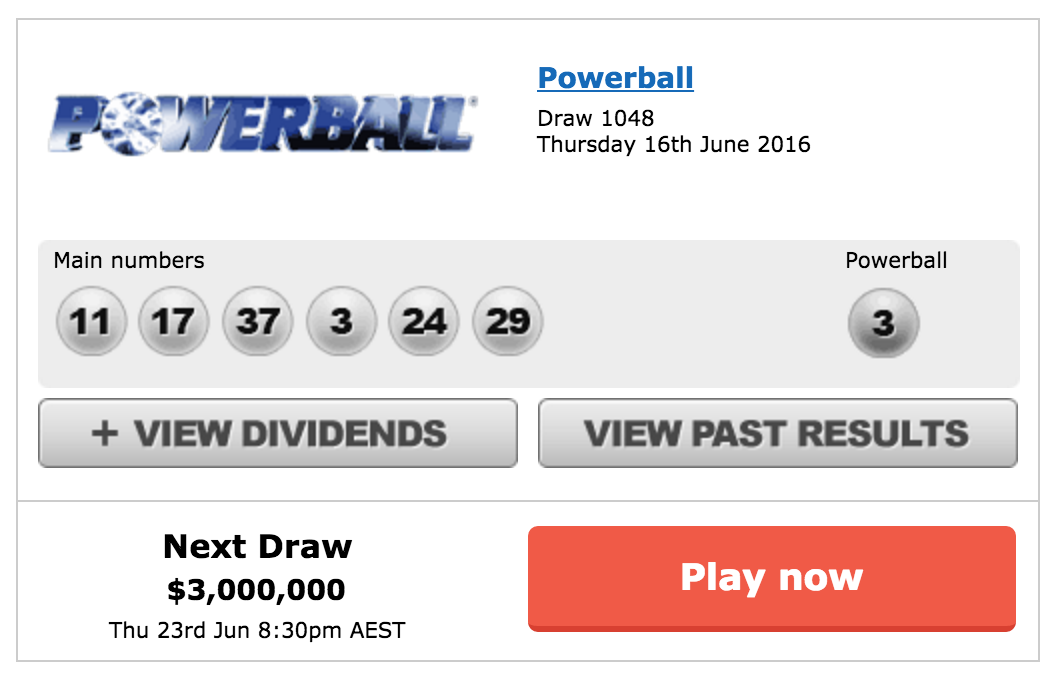
\includegraphics[height=3cm]{../images/Powerball.jpg}
\end{center}
\href{https://tatts.com/goldencasket/games/powerball/how-to-play}{\beamergotobutton{Powerball Rules}}

\end{frame}

\subsection{Example2: Tasmanian fruit flies}
\begin{frame}\frametitle{Example2: Tasmanian Fruit flies}

Tasmania is currently free of fruit fly which adds several million dollars to the annual export income earned by the horticultural industries. However the 14 species of fruit fly on the Australian mainland are a constant economic threat. South Australia remains the only Australian mainland state that is fruit fly free, with prevention, detection and eradication measures costing about \textdollar 5 million annually. 

\begin{center}
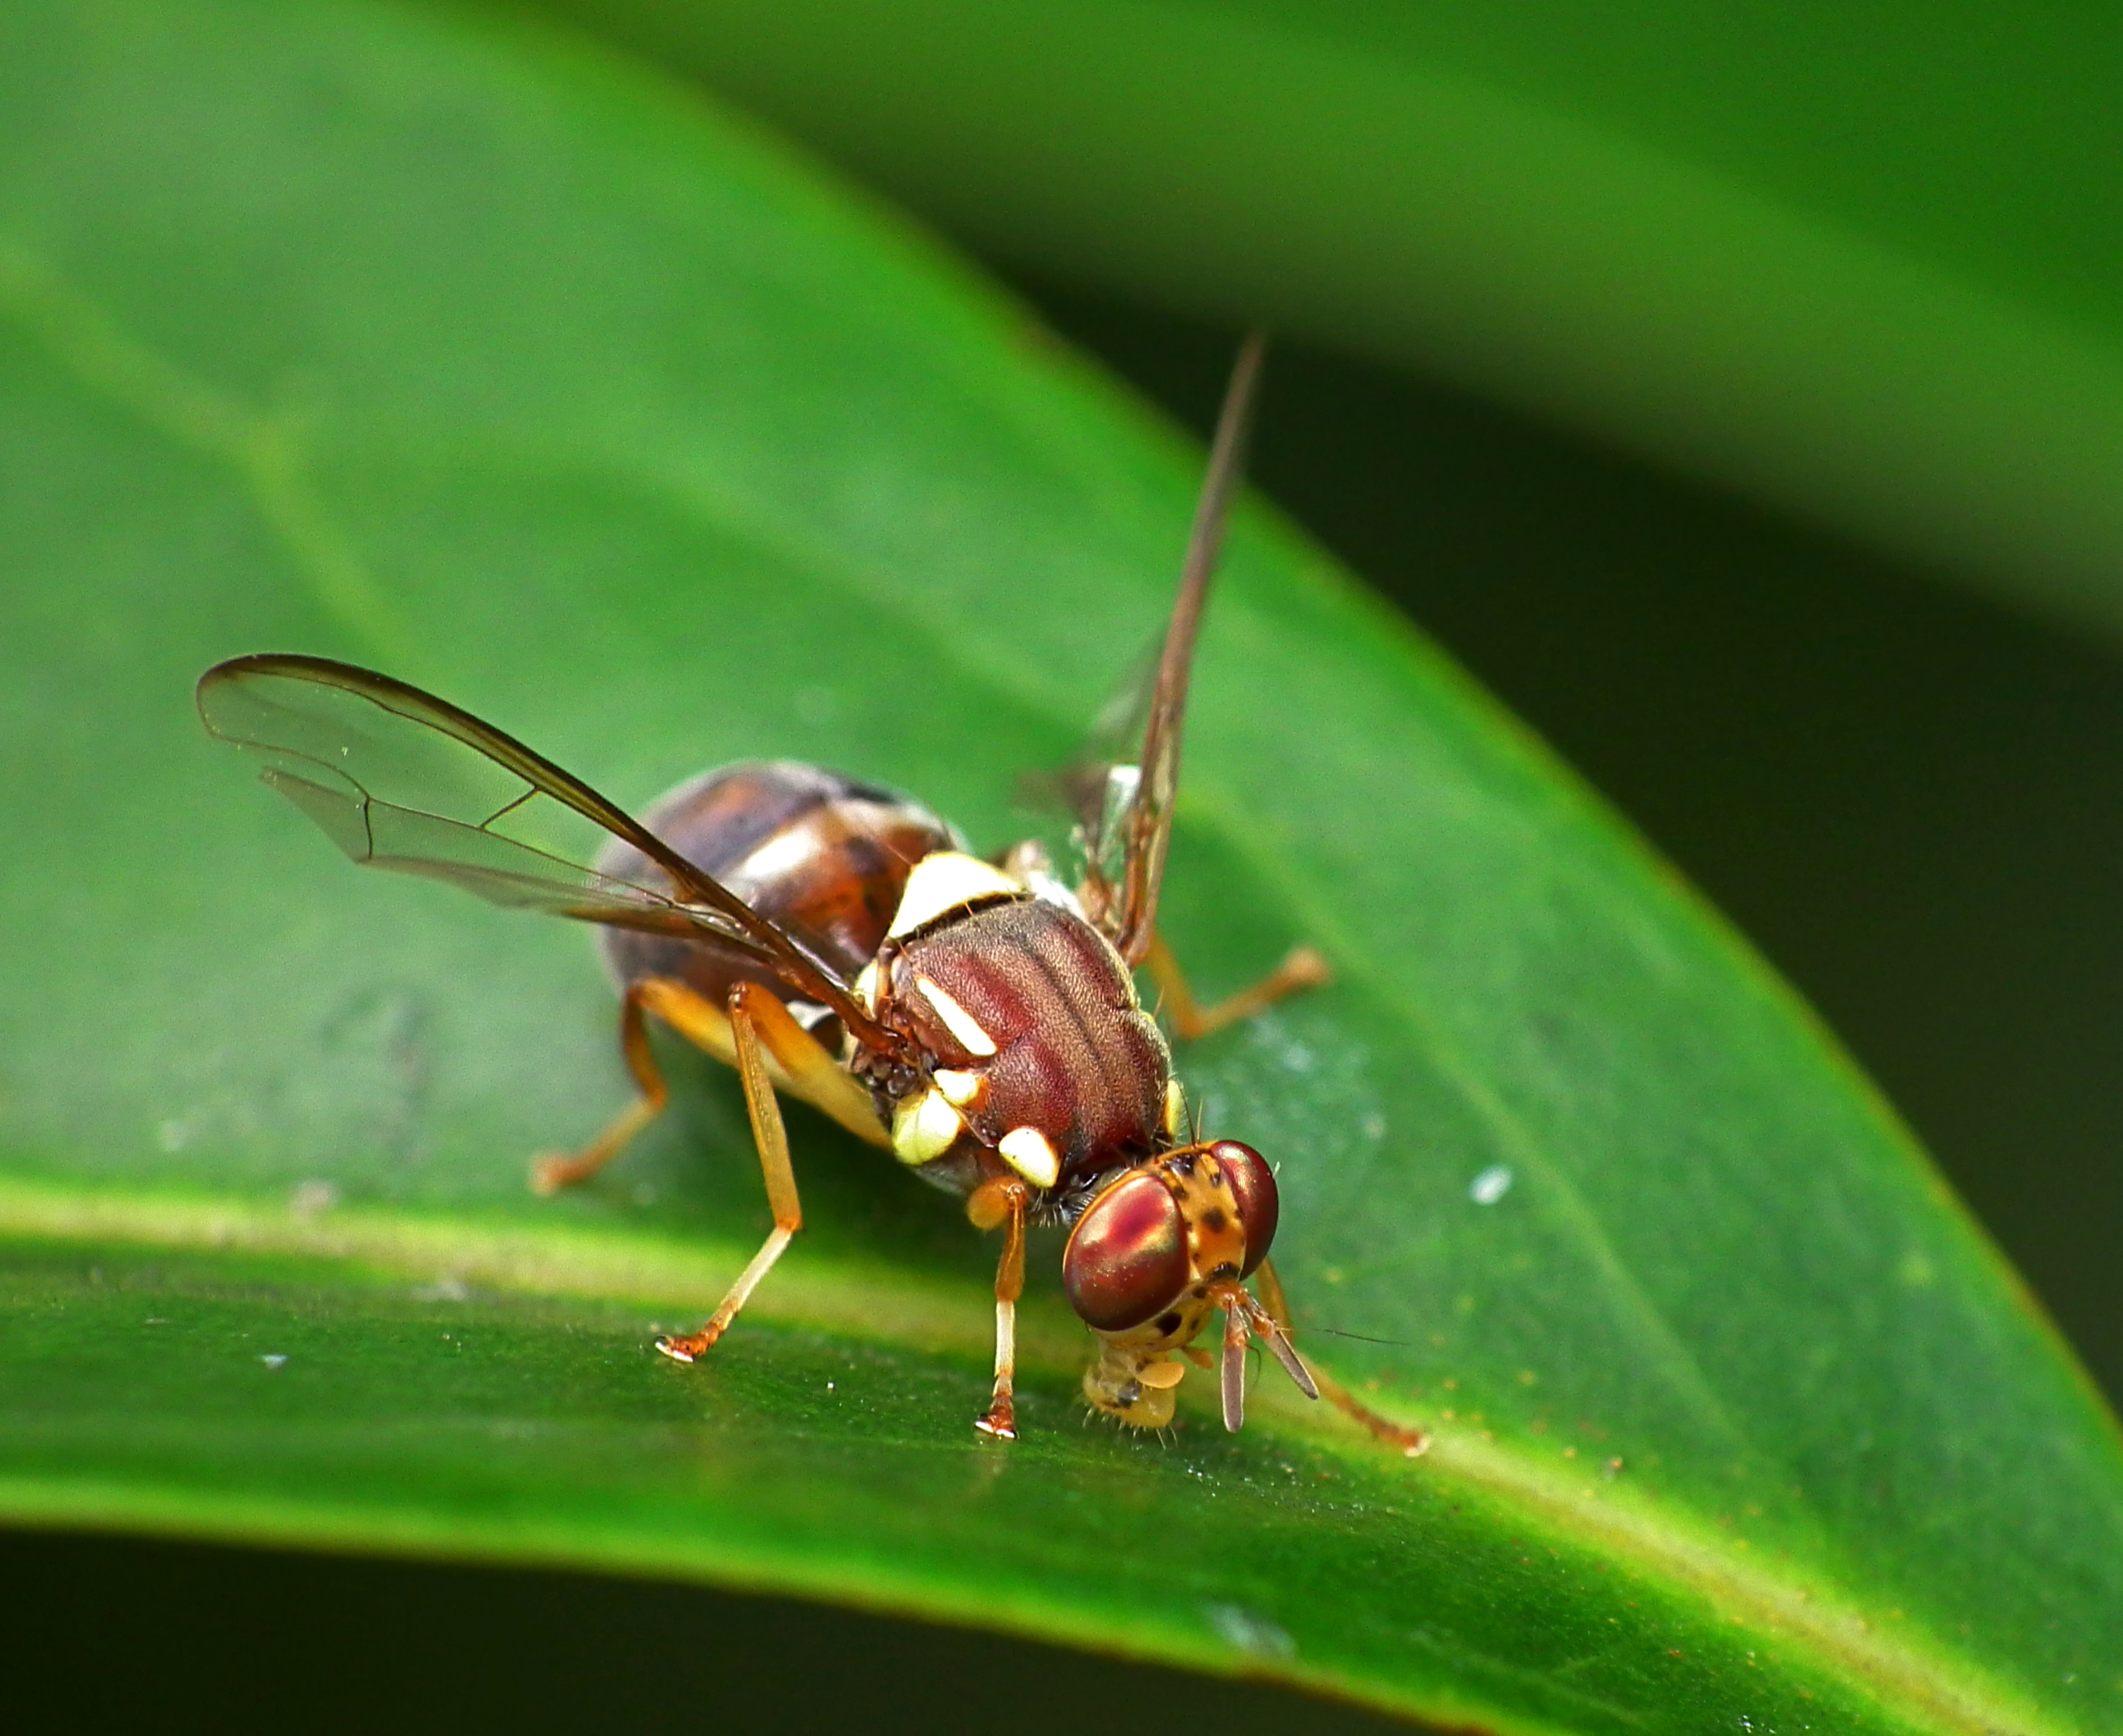
\includegraphics[height=3cm]{../images/Queensland_Fruit_Fly_-_Bactrocera_tryoni.jpg}
\end{center}
\href{http://dpipwe.tas.gov.au/biosecurity/plant-biosecurity/pests-and-diseases/fruit-fly}{\beamergotobutton{TasmaniaGovt}}
\href{http://pir.sa.gov.au/biosecurity/fruit\_fly}{\beamergotobutton{Biosecurity}}
\end{frame}

\begin{frame}\frametitle{}

Suppose there are 100 fruit flies buzzing around a lime tree. The flies have a 20\% chance on landing on the tree and act independently. 

\vspace{.5cm}
{\bf What is the probability that exactly 20 flies land on the lime tree?}

\vspace{1cm}
{\tiny Note: If there were only 2 flies, we could use simple probability.
\begin{itemize}
\item The set of all possible values: $x=0,1,2$.
\item  The likelihood of each value (discrete): \\
$P(X=0) = P(\mbox{no flies land}) = 0.8 \times 0.8 = 0.64$ \\
$P(X=1) = P(\mbox{1 fly lands}) = 0.2 \times 0.8 +  0.8 \times 0.2 = 0.32$ \\
$P(X=2) = P(\mbox{both flies land}) = 0.2^2  = 0.04$ \\
\end{itemize}

But we can't use this approach for a  realistic number of flies, like $n=100$. So we need to develop a general formula for $P(X=x)$.}
\end{frame}


\subsection{Example3: Calcium deficiency in orchards}
\begin{frame}\frametitle{Example3: Calcium deficiency in orchards}

While magnesium deficiency occurs in most districts in New South Wales, calcium deficiency is rarely seen in citrus orchards. A deficient range is below 1.6 percent of dry leaf matter and satisfactory range is 3-5.5.

\vspace{.5cm}
A small size orchard is considering ordering an expensive fertilizer. {\bf What is the chance that more than 1 tree will be calcium deficient?}

\vspace{.5cm}
\href{http://www.dpi.nsw.gov.au/agriculture/horticulture/citrus/management/nutrition/nutrition}{\beamergotobutton{NSW agriculture}}
\end{frame}


\subsection{Discrete Distributions}
\begin{frame}\frametitle{Discrete Distributions}
\begin{definition}[Discrete Distribution]

For any \alert{discrete} distribution $X$, we have a sample space $\Omega$ with values $x= \{ x_{1}, x_{2}, \ldots \}$ and associated probabilities $\{ p_{1}, p_{2} \ldots \}$, where $\{ p_{i} = P(X=x_{i}) \}$.

\vspace{.5cm}
Properties: 
\begin{itemize}
\item there is a countable number of possible values;
\item $\sum_{i} p_{i} = 1$
\end{itemize}
\end{definition}
\end{frame}

\begin{frame}\frametitle{}
\begin{definition}[Probability Distribution Function]
The probability distribution function (or probability distribution) of $X$ is 
the set of \{$x, P(X=x) \}$.
\end{definition}

\vspace{.5cm}
\begin{definition}[Cumulative Distribution Function (CDF)]

The cumulative distribution function (CDF) of $X$ is 
\[ F(x) = P(X \leq x) \]

This is a step function. Statistical tables are often presented in terms of the CDF.
\end{definition}
\end{frame}


\subsection{Mean and Variance of Discrete Distributions}
\begin{frame}\frametitle{The Mean of a Discrete Distribution}

\begin{definition}[Mean or Expectation]
The mean of $X$ is 
\[ \mu = E(X) = \sum_{x} x P(X=x)  \]

\end{definition}

\begin{definition}[Expectation of a Function]

The expectation of $g(X)$ is 
\[ E(g(X)) = \sum_{x} g(x) P(X=x)  \]

For example: $E(X^2) = \sum_{x} x^2 P(X=x) $.

\end{definition}

\end{frame}

\begin{frame}\frametitle{The Variance of a Discrete Distribution}
\begin{definition}[Variance]

The variance of $X$ is 
\[ Var(X) = V(X) =  E(X - \mu)^2 = E(X^2) - E(X)^2  \]
\end{definition}

\end{frame}


\begin{frame}\frametitle{What does the `Mean' mean?}

There are 4 main statistical usages of the word `mean':
\begin{itemize}
\item 
The mean of a sample: $\bar{x}$
\item
The mean of a population: $\mu$
\item
The mean of a random variable $X$ (describing a population): $E(X)$
\item
The distribution of the sampling mean: $\bar{X}$
\end{itemize}

\vspace{.5cm}
Similarly, there are 4 main usages of the word `variance'.

\end{frame}


\begin{frame}\frametitle{Example}
\begin{block}{Mean and variance of 5 tosses of a coin}
Let $X = $ the number of heads in 5 tosses of a coin, $x=0,1,\ldots,5$, with probability distribution function:

\begin{center}
\begin{tabular}{|l|l|l|l|l|l|l|} \hline
$x$ & 0 & 1 & 2 & 3 & 4 & 5  \\ \hline
$P(X=x)$ & $\frac{1}{32}$ & $\frac{5}{32}$ & $\frac{10}{32}$ & $\frac{10}{32}$ & $\frac{5}{32}$ & $\frac{1}{32}$  \\ \hline
\end{tabular}
\end{center}

Find the mean and variance of $X$.
\end{block}
\end{frame}

\begin{frame}\frametitle{}
\begin{alertblock}{}

\[ \mu = E(X) = \sum_{x} x P(X=x) = 0 \times \frac{1}{32} + 1 \times \frac{5}{32} + \ldots  5 \times \frac{1}{32} = 2.5 \]

\[ E(X^2) = \sum_{i} x^2 P(X=x) = 0^2 \times \frac{1}{32} + 1^2 \times \frac{5}{32} + \ldots  5^2 \times \frac{1}{32} = 7.5 \]

Hence
\[ Var(X) = E(X^2) - E(X)^2 = 7.5 - (2.5)^2 = 1.25  \]

\end{alertblock}
\end{frame}

\begin{frame}[fragile]\frametitle{In R}
\begin{knitrout}
\definecolor{shadecolor}{rgb}{0.969, 0.969, 0.969}\color{fgcolor}\begin{kframe}
\begin{alltt}
\hlstd{x}\hlkwb{=}\hlkwd{c}\hlstd{(}\hlnum{0}\hlstd{,}\hlnum{1}\hlstd{,}\hlnum{2}\hlstd{,}\hlnum{3}\hlstd{,}\hlnum{4}\hlstd{,}\hlnum{5}\hlstd{)}
\hlstd{p}\hlkwb{=}\hlkwd{c}\hlstd{(}\hlnum{1}\hlstd{,}\hlnum{5}\hlstd{,}\hlnum{10}\hlstd{,}\hlnum{10}\hlstd{,}\hlnum{5}\hlstd{,}\hlnum{1}\hlstd{)}\hlopt{/}\hlnum{32}
\hlkwd{sum}\hlstd{(x}\hlopt{*}\hlstd{p)}
\end{alltt}
\begin{verbatim}
## [1] 2.5
\end{verbatim}
\begin{alltt}
\hlkwd{sum}\hlstd{(x}\hlopt{^}\hlnum{2}\hlopt{*}\hlstd{p)}
\end{alltt}
\begin{verbatim}
## [1] 7.5
\end{verbatim}
\begin{alltt}
\hlkwd{sum}\hlstd{(x}\hlopt{^}\hlnum{2}\hlopt{*}\hlstd{p)}\hlopt{-}\hlstd{(}\hlkwd{sum}\hlstd{(x}\hlopt{*}\hlstd{p))}\hlopt{^}\hlnum{2}
\end{alltt}
\begin{verbatim}
## [1] 1.25
\end{verbatim}
\begin{alltt}
\hlkwd{sum}\hlstd{((x}\hlopt{-}\hlkwd{sum}\hlstd{(x}\hlopt{*}\hlstd{p))}\hlopt{^}\hlnum{2}\hlopt{*}\hlstd{p)}
\end{alltt}
\begin{verbatim}
## [1] 1.25
\end{verbatim}
\end{kframe}
\end{knitrout}
\end{frame}

\begin{frame}[fragile]\frametitle{}
\begin{alertblock}{Have a try}
In a certain game, 5 coins are tossed, where $X$ denotes the number of heads. It costs \$8.00 to play, and the player receives $\$ 2^X$ as prize money. Show that the expected loss for 1 game is $\$ 0.41$.
\end{alertblock}

\begin{knitrout}
\definecolor{shadecolor}{rgb}{0.969, 0.969, 0.969}\color{fgcolor}\begin{kframe}
\begin{alltt}
\hlcom{#Check your answer}
\hlstd{x}\hlkwb{=}\hlkwd{c}\hlstd{(}\hlnum{0}\hlstd{,}\hlnum{1}\hlstd{,}\hlnum{2}\hlstd{,}\hlnum{3}\hlstd{,}\hlnum{4}\hlstd{,}\hlnum{5}\hlstd{)}
\hlstd{p}\hlkwb{=}\hlkwd{c}\hlstd{(}\hlnum{1}\hlstd{,}\hlnum{5}\hlstd{,}\hlnum{10}\hlstd{,}\hlnum{10}\hlstd{,}\hlnum{5}\hlstd{,}\hlnum{1}\hlstd{)}\hlopt{/}\hlnum{32}
\hlkwd{sum}\hlstd{((}\hlnum{2}\hlopt{^}\hlstd{x)}\hlopt{*}\hlstd{p)}\hlopt{-}\hlnum{8.00}
\end{alltt}
\begin{verbatim}
## [1] -0.40625
\end{verbatim}
\end{kframe}
\end{knitrout}
\end{frame}


\begin{frame}[fragile]{}
\begin{alertblock}{Your Turn}
Suppose you toss a fair coin 1000 times:  when it lands heads
you receive \$1, and when it lands tails you pay me \$1.
What is your expected profit or loss?
\end{alertblock}


\begin{knitrout}
\definecolor{shadecolor}{rgb}{0.969, 0.969, 0.969}\color{fgcolor}\begin{kframe}
\begin{alltt}
\hlstd{x}\hlkwb{=}\hlkwd{c}\hlstd{(}\hlnum{1}\hlstd{,}\hlopt{-}\hlnum{1}\hlstd{)}
\hlstd{p}\hlkwb{=}\hlkwd{c}\hlstd{(}\hlnum{0.5}\hlstd{,}\hlnum{0.5}\hlstd{)}
\hlkwd{sum}\hlstd{(x}\hlopt{*}\hlstd{p)}
\end{alltt}
\begin{verbatim}
## [1] 0
\end{verbatim}
\end{kframe}
\end{knitrout}
\end{frame}


\subsection{Example1: Hypergeometric Distribution}

\begin{frame}\frametitle{Common Types of Discrete Distributions}
There are an infinite number of discrete distributions. 

\vspace{0.5cm}
We will concentrate on 2 special examples: 
\begin{itemize}
\item The Hypergeometric Distribution (Urn model);
\item The Binomial Distribution;
\end{itemize}

For your reference, the Poisson Distribution is also considered as an Appendix.
\end{frame}

\begin{frame}[fragile]{Example1: Hypergeometric Distribution}

\begin{definition}[General Hypergeometric Model]
The \alert{Hypergeometric distribution} models a context described by an urn model.

\vspace{.5cm}
Suppose an urn contains $N$ balls, with $N_{1}$ of type 1, $N_{2}$ of type 2, $\ldots$ $N_{k}$ of type $k$, where $\sum_{i=1}^{k} N_{i} = N$.

\vspace{.5cm}
We select a random sample (without replacement) of $n$ balls (where $n \leq N$.)

\vspace{.5cm}
The probability that we select exactly $n_{i}$ of type $i$ is 

\[ P( \mbox{Select $n_{i}$ balls of each type $i$} )   = 
\frac{ { N_{1} \choose n_{1}}  {N_{2} \choose n_{2}} \ldots {N_{k} \choose n_{k}}  }{ {N \choose n} }
\]

\end{definition}
\hyperlink{Factorials}{\beamergotobutton{Factorials}}
\hyperlink{BinomialCoefficients}{\beamergotobutton{BinomialCoefficients}}
\end{frame}

\begin{frame}[fragile]{}

\begin{block}{Example (Packet of M \& Ms)}
Suppose a small Christmas packet of M \& Ms contains $16$ chocolates, of which  $10$ are red and $6$ are green. We select a random sample of $3$ chocolates. What is the probability of selecting exactly $2$ red ones?
\end{block}

\begin{center}
\begin{tikzpicture}
\draw [blue] (0,1) rectangle (6.1,2);
\draw [red, fill=red, ultra thick] (0.6,1.5) circle [radius=0.1];;
\draw [red, fill=red, ultra thick] (0.9,1.5) circle [radius=0.1];;
\draw [red, fill=red, ultra thick] (1.2,1.5) circle [radius=0.1];;
\draw [red, fill=red, ultra thick] (1.5,1.5) circle [radius=0.1];;
\draw [red, fill=red, ultra thick] (1.8,1.5) circle [radius=0.1];;
\draw [red, fill=red, ultra thick] (2.1,1.5) circle [radius=0.1];;
\draw [red, fill=red, ultra thick] (2.4,1.5) circle [radius=0.1];;
\draw [red, fill=red, ultra thick] (2.7,1.5) circle [radius=0.1];;
\draw [red, fill=red, ultra thick] (3,1.5) circle [radius=0.1];;
\draw [red, fill=red, ultra thick] (3.3,1.5) circle [radius=0.1];;
\draw [green, fill=green, ultra thick] (4,1.5) circle [radius=0.1];;
\draw [green, fill=green, ultra thick] (4.3,1.5) circle [radius=0.1];;
\draw [green, fill=green, ultra thick] (4.6,1.5) circle [radius=0.1];;
\draw [green, fill=green, ultra thick] (4.9,1.5) circle [radius=0.1];;
\draw [green, fill=green, ultra thick] (5.2,1.5) circle [radius=0.1];;
\draw [green, fill=green, ultra thick] (5.5,1.5) circle [radius=0.1];;

\draw [->, blue, ultra thick]  (3,1) -- (3,0);

\draw [blue, rounded corners=.8ex] (2,-1) rectangle (4,0);
\draw [red, fill=red, ultra thick] (2.3,-0.5) circle [radius=0.1];;
\draw [red, fill=red, ultra thick] (2.6,-0.5) circle [radius=0.1];;
\draw [green, fill=green, ultra thick] (3.3,-0.5) circle [radius=0.1];;
\end{tikzpicture}
\end{center}

The probability that we select exactly $n=2$ red balls is
\[ \frac{ { 10 \choose 2}  {6 \choose 1}  }{ {16 \choose 3} } \approx 0.48 \]

\end{frame}

\begin{frame}[fragile]{}
\begin{knitrout}
\definecolor{shadecolor}{rgb}{0.969, 0.969, 0.969}\color{fgcolor}\begin{kframe}
\begin{alltt}
\hlkwd{choose}\hlstd{(}\hlnum{10}\hlstd{,}\hlnum{2}\hlstd{)}\hlopt{*}\hlkwd{choose}\hlstd{(}\hlnum{6}\hlstd{,}\hlnum{1}\hlstd{)}\hlopt{/}\hlkwd{choose}\hlstd{(}\hlnum{16}\hlstd{,}\hlnum{3}\hlstd{)}
\end{alltt}
\begin{verbatim}
## [1] 0.4821429
\end{verbatim}
\end{kframe}
\end{knitrout}

\begin{knitrout}
\definecolor{shadecolor}{rgb}{0.969, 0.969, 0.969}\color{fgcolor}\begin{kframe}
\begin{alltt}
\hlkwd{dhyper}\hlstd{(}\hlnum{2}\hlstd{,}\hlnum{10}\hlstd{,}\hlnum{6}\hlstd{,}\hlnum{3}\hlstd{)}   \hlcom{# dhyper(x,N1,N2,n)}
\end{alltt}
\begin{verbatim}
## [1] 0.4821429
\end{verbatim}
\end{kframe}
\end{knitrout}

\end{frame}

\begin{frame}[fragile]{}
\begin{block}{Example (Powerball)}
What is the probability of winning Powerball (Division 1)?  
\end{block}

\begin{knitrout}
\definecolor{shadecolor}{rgb}{0.969, 0.969, 0.969}\color{fgcolor}\begin{kframe}
\begin{alltt}
\hlstd{(}\hlkwd{choose}\hlstd{(}\hlnum{6}\hlstd{,}\hlnum{6}\hlstd{)}\hlopt{*}\hlkwd{choose}\hlstd{(}\hlnum{34}\hlstd{,}\hlnum{0}\hlstd{)}\hlopt{/}\hlkwd{choose}\hlstd{(}\hlnum{40}\hlstd{,}\hlnum{6}\hlstd{))}\hlopt{*}
  \hlstd{(}\hlkwd{choose}\hlstd{(}\hlnum{1}\hlstd{,}\hlnum{1}\hlstd{)}\hlopt{*}\hlkwd{choose}\hlstd{(}\hlnum{19}\hlstd{,}\hlnum{0}\hlstd{)}\hlopt{/}\hlkwd{choose}\hlstd{(}\hlnum{20}\hlstd{,}\hlnum{1}\hlstd{))}
\end{alltt}
\begin{verbatim}
## [1] 1.302633e-08
\end{verbatim}
\end{kframe}
\end{knitrout}

\begin{knitrout}
\definecolor{shadecolor}{rgb}{0.969, 0.969, 0.969}\color{fgcolor}\begin{kframe}
\begin{alltt}
\hlkwd{dhyper}\hlstd{(}\hlnum{6}\hlstd{,}\hlnum{6}\hlstd{,}\hlnum{34}\hlstd{,}\hlnum{6}\hlstd{)}\hlopt{*}\hlkwd{dhyper}\hlstd{(}\hlnum{1}\hlstd{,}\hlnum{1}\hlstd{,}\hlnum{19}\hlstd{,}\hlnum{1}\hlstd{)}
\end{alltt}
\begin{verbatim}
## [1] 1.302633e-08
\end{verbatim}
\end{kframe}
\end{knitrout}

\vspace{.5cm}
Does this match the claim on the powerball website?
`The chance of winning a Division One prize in Powerball is 1 in 76,767,600'.
\href{https://www.ozlotteries.com/play/powerball}{\beamergotobutton{Powerball Rules}}

\end{frame}

\subsection{Example2: Binomial Distribution}
\begin{frame}\frametitle{Example2: Binomial Distribution}
\begin{definition}[Binomial Distribution]
The \alert{Binomial distribution} models a context in which we have:
\begin{itemize}
\item a fixed number $n$ of independent Binary trials; 
\item  a fixed likelihood of a success at each trial $p=P(\mbox{success})$. 
\end{itemize}

\vspace{.5cm}
If $X =$ the number of successes in $n$ trials, then  $X \sim Bin(n,p)$ with
\[ P(X=x) = {n \choose x} p^x (1-p)^{n-x} \hspace{1cm} \mbox{for } x=0,1,2,\ldots,n. \]
\end{definition}

\vspace{.5cm}
Note:  $\sim$ reads `is distributed as'.
\hyperlink{Factorials}{\beamergotobutton{Factorials}}
\hyperlink{BinomialCoefficients}{\beamergotobutton{BinomialCoefficients}}
\end{frame}

\begin{frame}
Notes:
\begin{itemize}
\item A {\it Binary} (or Bernoulli) trial is an event where there can only be 2 options: success or failure. For example, 1 fruit fly is buzzing around a fruit tree: will it land or not?
\item {\it Success} designates the event we are interested in counting, which may not be good. For example,  $p=P(\mbox{fruit fly lands on fruit tree})$.
\item The Binomial distribution has 2 parameters: $n$ and $p$. Parameters represent the numerical inputs needed for the model.
\item It can be shown (by algebra) that the Binomial distribution has mean $E(X)=np$ and variance $Var(X)=np(1-p)$.
\end{itemize}
\end{frame}

\begin{frame}[fragile]\frametitle{Example of Binomial Distribution with changing $p$}

$X \sim Bin(n=20,p)$, for different $p=0.1,0.2,\ldots ,1$. \\

\vspace{0.5cm}
\begin{knitrout}
\definecolor{shadecolor}{rgb}{0.969, 0.969, 0.969}\color{fgcolor}
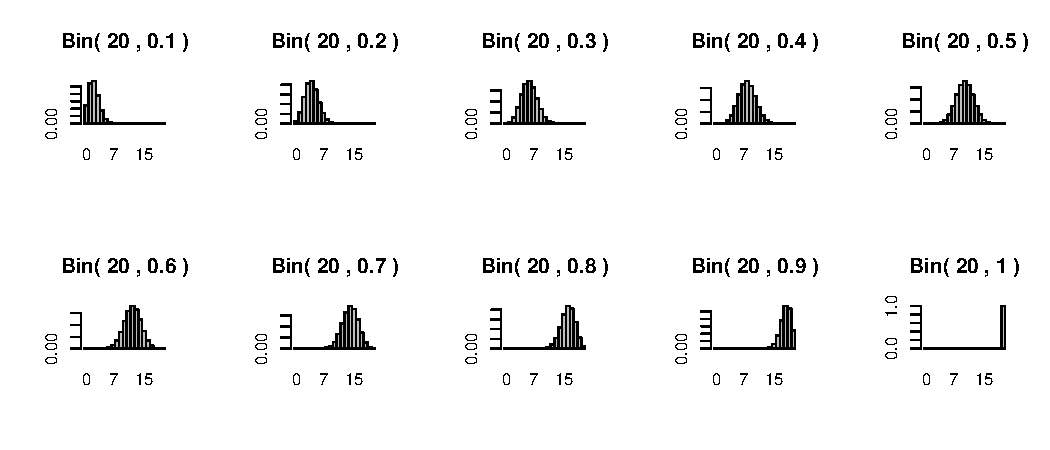
\includegraphics[width=\maxwidth]{figure/unnamed-chunk-9-1} 

\end{knitrout}

\end{frame}



\begin{frame}\frametitle{Example}
\begin{block}{Fruit Flies}
There are 10 fruit flies buzzing around a lime tree. The flies have a 20\% chance on landing on the tree and act independently.
If $X$ represents the number of flies that land on the tree, what is the distribution of $X$?  What is the chance that no flies land on the tree? What is the chance that less than 2 flies land on the tree? 

\vspace{.5cm}
\begin{enumerate}
\item Identify the model: \\
$X = \mbox{the number of flies that land} \sim Bin(n,p)$, where
$n= \mbox{number of flies} = 10$;
$p=P(\mbox{fruit fly lands}) =0.2$.
\item  
Calculate probability:\\
$P(\mbox{no flies land}) = P(X=0) = {10 \choose 0} (0.2)^0 (0.8)^{10} = \frac{10!}{0! (10-0)!} (0.8)^{10} =(0.8)^{10} \approx 0.11$.
\end{enumerate}
\end{block}
\end{frame}


\begin{frame}[fragile]\frametitle{}
\begin{block}{}
Calculate probability:  \\
$P(\mbox{less than 2 flies land}) = P(X \leq 1) = P(X=0) +P(X=1) = 0.1073742 + {10 \choose 1} (0.2)^1 (0.8)^9 \approx 0.38$.
\end{block}

\begin{knitrout}
\definecolor{shadecolor}{rgb}{0.969, 0.969, 0.969}\color{fgcolor}\begin{kframe}
\begin{alltt}
\hlcom{# dbinom(x,n,p) calculates P(X=x) for Bin(n,p)}
\hlkwd{dbinom}\hlstd{(}\hlnum{0}\hlstd{,}\hlnum{10}\hlstd{,}\hlnum{0.2}\hlstd{)}
\end{alltt}
\begin{verbatim}
## [1] 0.1073742
\end{verbatim}
\end{kframe}
\end{knitrout}

\begin{knitrout}
\definecolor{shadecolor}{rgb}{0.969, 0.969, 0.969}\color{fgcolor}\begin{kframe}
\begin{alltt}
\hlcom{# pbinom(x,n,p) calculates P(X<=x) for Bin(n,p)}
\hlkwd{pbinom}\hlstd{(}\hlnum{1}\hlstd{,}\hlnum{10}\hlstd{,}\hlnum{0.2}\hlstd{)}
\end{alltt}
\begin{verbatim}
## [1] 0.3758096
\end{verbatim}
\end{kframe}
\end{knitrout}
\end{frame}


\subsection{Appendix: Poisson Distribution}
\begin{frame}\frametitle{Appendix: Poisson Distribution}

The Poisson distribution is used in 2nd year courses, so is given here for reference.

\begin{definition}[Poisson Distribution]
The \alert{Poisson distribution} models a context in which we have
\begin{itemize}
\item events occuring in an interval; 
\item the average number of events occuring in an interval is $\lambda$ (rate).
\end{itemize}

\vspace{.5cm}
If $X =$ number of events in the interval, then $X \sim Po(\lambda)$ and

\[ P(X=x) =   \frac{ \lambda^x e^{-\lambda}}{x!} 
\hspace{1cm} \mbox{for } x=0,1,2,\ldots \mbox{ and } \lambda > 0. \]
\end{definition}
\end{frame}

\begin{frame}
Notes:
\begin{itemize}
\item $\lambda$ is pronounced `lambda'.
\item Poisson is pronounced `pwasonn'.
\item The Poisson distribution has 1 parameter: $\lambda$.
\item 
The Poisson Distribution models rare events, where $\lambda$ is small.

For example, $\lambda=$ the average number of lime trees exhibiting calcium deficiency in an orchard in a year.
\item It can be shown (by algebra) that the Poisson distribution has mean $E(X)=Var(X)=\lambda.$
\end{itemize}

\vspace{.5cm}
Extension: For large $n$ and small $p$, $X \sim Bin(n,p)$ can be approximated by $Y \sim Po(\lambda=np)$.
\end{frame}

\begin{frame}[fragile]\frametitle{Examples of Poisson Distributions with changing $\lambda$}

$X \sim P_{0}(\lambda)$, for different $\lambda=1,0.2,\ldots 10$. \\

\vspace{0.5cm}
\begin{knitrout}
\definecolor{shadecolor}{rgb}{0.969, 0.969, 0.969}\color{fgcolor}
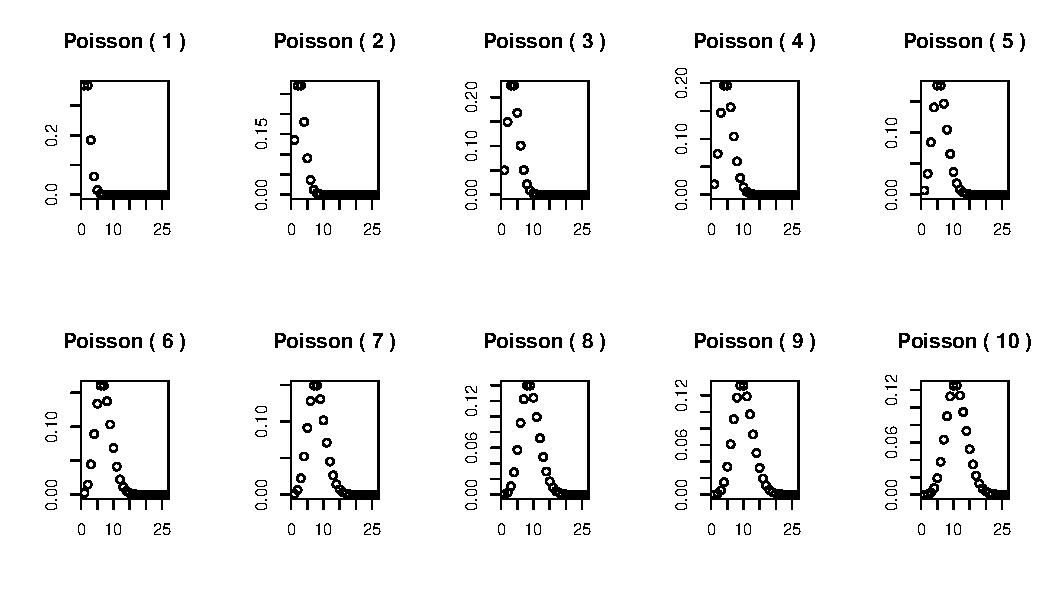
\includegraphics[width=\maxwidth]{figure/unnamed-chunk-12-1} 

\end{knitrout}
\end{frame}

\begin{frame}\frametitle{Example}
\begin{block}{Magnesium deficiency}

While magnesium deficiency occurs in most districts in New South Wales, calcium deficiency is rarely seen in citrus orchards. A deficient range is below 1.6 percent of dry leaf matter and satisfactory range is 3-5.5.

\vspace{.5cm}
For a small size orchard, let $X$ represent the number of trees with calcium deficiency in a year, where $\lambda=2$.  
For ordering an expensive fertilizer, what is the chance that more than 1 tree will be calcium deficient? 
\href{http://www.dpi.nsw.gov.au/agriculture/horticulture/citrus/management/nutrition/nutrition}{\beamergotobutton{NSW agriculture}}
\end{block}
\end{frame}

\begin{frame}\frametitle{}


\begin{block}{}
\begin{enumerate}
\item Identify the model: \\
$X = \mbox{the number of trees that are calcium deficient} \sim Po(\lambda)$, where 
$\lambda= \mbox{average number of deficient trees in a year} = 2$.
\item  
Calculate probabilities: \\
$P(\mbox{X=0}) = \frac{ 2^0 e^{-2}}{0!} =e^{-2} = 0.1353353$ \\
$P(\mbox{X = 1}) =  \frac{ 2^1 e^{-2}}{1!} = 0.2706706$ \\
$P(X > 1) = 1- P(X=0) - P(X=1) = 0.5939941$
\end{enumerate}
\end{block}
\end{frame}

\begin{frame}[fragile]\frametitle{}
\begin{knitrout}
\definecolor{shadecolor}{rgb}{0.969, 0.969, 0.969}\color{fgcolor}\begin{kframe}
\begin{alltt}
\hlcom{# dpois(x,l) calculates P(X=x) for Po(l)}

\hlkwd{dpois}\hlstd{(}\hlnum{0}\hlstd{,}\hlnum{2}\hlstd{)}
\end{alltt}
\begin{verbatim}
## [1] 0.1353353
\end{verbatim}
\end{kframe}
\end{knitrout}

\begin{knitrout}
\definecolor{shadecolor}{rgb}{0.969, 0.969, 0.969}\color{fgcolor}\begin{kframe}
\begin{alltt}
\hlcom{# ppois(x,l) calculates P(X<=x) for Po(l)}

\hlnum{1}\hlopt{-}\hlkwd{ppois}\hlstd{(}\hlnum{1}\hlstd{,}\hlnum{2}\hlstd{)}
\end{alltt}
\begin{verbatim}
## [1] 0.5939942
\end{verbatim}
\end{kframe}
\end{knitrout}
\end{frame}

\end{document}
